\chapter{WordNet e FrameNet}

\section{WordNet}

\dfn{WordNet}{
  WordNet è un sistema di riferimenti lessicali online il cui design è ispirato dalle teorie psicolinguistiche sulla memoria lessicale umana. Nomi, verbi e aggettivi sono organizzati in insiemi di sinonimi ognuno rappresentante uno specifico concetto lessicale.
}

\paragraph{Problemi dei dizionari "classici":}

\begin{itemize}
  \item Vengono messe insieme parole che sono simili per posizionamento di letter. 
  \item Parole con significati simili o collegati sono molto sparse. 
  \item Non esiste un'alternativa ovvia per permettere al lettore di cercare una specifica parola.
\end{itemize}

\nt{Per i computer è molto facile cercare in pochi istanti tra migliaia di termini, ma sarebbe uno spreco limitarsi a quello.}

\paragraph{1985, Princeton:}

\begin{itemize}
  \item Un gruppo di psicologi e linguisti inizia sviluppare un database lessicale.  
  \item L'idea iniziale era quella di fornire un aiuto nella ricerca nei dizionari a livello \fancyglitter{concettuale}. 
  \item Avrebbe dovuto essere usato in congiunzione con un dizionario online convenzionale.
\end{itemize}

\paragraph{WordNet divide il lessico in 4 categorie:}

\begin{itemize}
  \item Nomi: organizzati come gerarchie.
  \item Verbi: organizzati come una serie di relazioni.
  \item Aggettivi. 
  \item Avverbi.
\end{itemize}

\subsection{La Matrice Lessicale}

\dfn{Parola}{
  Una parola è un'associazione convenzionale tra un concetto lessicalizzato e un'espressione (utterance) sintattica. Per ridurre l'ambuguità si utilizzano i termini:
  \begin{itemize}
    \item Word form: per riferirsi all'espressione fisica. 
    \item Word meaning: per riferirsi al concetto lessicalizzato espresso dalla forma.
  \end{itemize}
}

\paragraph{Matrice lessicale:}

\begin{itemize}
  \item La word form rappresenta le colonne. 
  \item Il word meaning rappresenta le righe.
  \item Se due entry sono nella stessa colonna le parole sono \fancyglitter{polisemiche}. 
  \item Se due entry sono nella stessa riga le parole sono \fancyglitter{sinonimi}.
\end{itemize}

\begin{figure}[h]
    \centering
    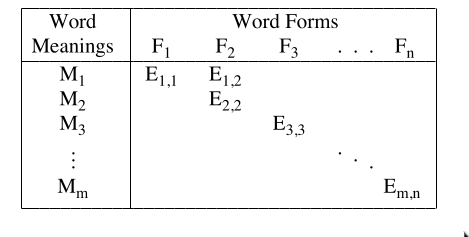
\includegraphics[scale=0.8]{03/matrix.png}
    \caption{Matrice lessicale.}
\end{figure}


\dfn{Synsets}{
  Il significato della parola $M_1$ può essere usato semplicamente scegliendo una forma $F_n$ che la esprime.
} 

\nt{Le persone che conoscono l'inglese hanno già assimilato i concetti e ci si aspetta che siano in grado di riconoscerli dalla parole appartenenti a un synset.}

\cor{Gloss}{
Breve definizione o descrizione del senso di una parola. Se non sono presenti sinonimi il gloss funziona da synset.
}

\subsection{Relazioni Semantiche}

WordNet è organizzato con \fancyglitter{relazioni semantiche}. Una relazione semantica è una relazione tra significati (rappresentati da synsets). In altre parole sono dei puntatori tra synsets. Una loro caratteristica è che sono simmetriche. 

\paragraph{Relazioni:}

\begin{itemize}
  \item \fancyglitter{Sinonimia:} relazione lessicale, similarità di significati. Due espressioni sono sinonimi se sostituendo l'una con l'altra non cambia il valore della frase. Tuttavia i veri sinonimi sono rari per cui si fa sempre riferimento a un determinato contesto linguistico.
  \item \fancyglitter{Antonimia:} è una relazione lessicale tra le forme delle parole, ma non tra i significati delle stesse. Per esempio "ricco" è antonimo di "povero", ma non sono opposti. "Ascesa" e "caduta" sono opposti, ma non sono antonimi.
  \item \fancyglitter{Iponimia:} relazione semantica del tipo ako (a kind of). È una relazione transitiva e asimmetrica.
  \item \fancyglitter{Meronimia:} relazione \fancyglitter{hasa} (part-whole). Anche questa relazione è transitiva e asimmetrica.
\end{itemize}

\subsection{Sostantivi}

I \fancyglitter{nomi} in WordNet sono organizzati in definizioni che forniscono un termine sopraordinato e alcune caratteristiche: 
\begin{itemize}
  \item Attributi. 
  \item Parti (meronimia). 
  \item Funzioni.
\end{itemize}

\paragraph{Le definizioni:}

\begin{itemize}
  \item Non specificano quale senso di un termine sopraordinato sia quello appropriato. 
  \item Non forniscono informazioni su termini coordinati. 
  \item Le definizioni puntano verso l'alto, non in termini laterali o in iponimi. 
  \item Un problema dei dizionari sono le definizioni circolarin ($w-a$ per definire $w_b$ e $w_b$ per definire $w_a$). In WordNet si è imposta una struttura ad albero per evitare questo.
\end{itemize}

\dfn{Assunzione Psicolinguistica}{
  La decisione di organizzare i nomi come un sistema di ereditarietà riflette un giudizio psicolinguistico sul lessico mentale. Ci sono evidenze che una struttura gerarcica sia più facile da concettualizzare.
}

\paragraph{Superordinati:}

\begin{itemize}
  \item I nomi superordinati possono servire come anafore per riferirsi ai loro iponimi. 
  \item I superordinati e i loro iponimi non possono essere confrontati. 
  \item Spiegazioni in termini di gerarchie di relazioni semantiche.
\end{itemize}

\paragraph{Evidenza sperimentale:}

\begin{itemize}
  \item Il \fancyglitter{tempo di reazione} può essere usato per indicare il numero di livelli gerarchici separanti due significati. 
  \item Esempio: le persone rispondo più in fretta a "un canarino può cantare" rispetto a "un canarino può volare". 
  \item Il tempo di reazione varia perché è richiesto tempo extra per estrarre caratteristiche da concetti sopraordinati.
\end{itemize}

\paragraph{Problemi aperti:}

\begin{itemize}
  \item L'informazione generica è ereditata oppure è "salvata" in modo ridondante?
  \item Alcuni termini condividono lo stesso collegamento semantico, ma alcuni vengono confermarti più rapidamente rispetto ad altri. 
  \item Ma se la memoria semantica non è organizzata come un sistema di eredità allora come? 
    \begin{itemize}
      \item L'assunzione di ineritanza è corretta, ma il tempo di reazione misura una distanza \fancyglitter{pragmatica}, non semantica.
    \end{itemize}
\end{itemize}

\paragraph{In WordNet:}

\begin{itemize}
  \item I nomi sono divisi in insiemi semantici che selezionano un certo numero picccolo di concetti e ognuno funziona da punto iniziale di una gerarchia (\fancyglitter{ereditarietà multipla}). 
  \item Ci sono 25 di questi "punti iniziali".
  \item Concetti generici: 
    \begin{itemize}
      \item Le gerarchie di nomi hanno un livello, nel mezzo, dove la maggior parte delle caratteristiche sono attaccate (basic-level). 
      \item Sopra il livello base i concetti sono brevi e generali. 
      \item Sotto il livello base ci sono cose più specifiche.
    \end{itemize}
  \item Caratteristiche: 
    \begin{itemize}
      \item La struttura è generata da relazioni di iponimi e i dettagli sono dati dalle caratteristiche che distinguono i concetti. 
      \item Esistono 3 tipi di caratteristiche: attributi (aggettivi), parti (nomi), funzioni (verbi). 
    \end{itemize}
\end{itemize}

\paragraph{Le caratteristiche:}

\begin{itemize}
  \item \fancyglitter{Attributi:}
    \begin{itemize}
      \item Il valore è espresso dagli aggettivi. 
      \item Gli aggettivi \evidence{modificano} il significato dei nomi. 
      \item Gli attributi associati a un nome si riflettono negli aggettivi che possono normalmente modificare quel nome.
    \end{itemize}
  \item \fancyglitter{Parti:}
    \begin{itemize}
      \item La relazione part-whole tra nomi (meronimia). 
      \item La meronimia ha una relazione inversa: se $w_m$ è un meronimo di $w_h$ allora $w_h$ è un olonimo di $w_m$.
      \item I meronimi sono caratteristiche distintive che gli iponimi possono ereditare e sono asimmetrici e transitivi (in maniera limitata). 
    \end{itemize}
  \item \fancyglitter{Funzioni:}
    \begin{itemize}
      \item Sono descrizioni di qualcosa che le istanze di un concetto fanno normalmente. 
      \item Tutte le caratteristiche dei nomi che sono descritte da verbi o frasi verbali. 
      \item Ci sono motivazioni linguistiche per cui si assume che una funzione è una caratteristica del significato. 
      \item Un oggetto che non è $X$ non può essere un buon $X$ se fa bene una funzione che viene effettuata normalmente da $X$. 
    \end{itemize}
\end{itemize}

\subsection{Verbi}

\dfn{Verbi}{
  I verbi forniscono un framework relazionale e semantico per le frasi. 
}

\paragraph{Sottocategorizzazioni:}

\begin{itemize}
  \item Strutture sintattiche che specificano quanti e quali tipi di argomenti un verbo può avere. 
  \item Ogni argomento ha un ruolo semantico, una funzione del significato dell'azione. 
  \item \fancyglitter{selectional restrictions:} specificano le proprietà semantiche di una classe di nomi. 
  \item Tutto ciò fa parte della voce del verbo in un dizionario mentale.
\end{itemize}

\clm{}{}{
  \begin{itemize}
    \item Ci sono molti meno verbi rispetto ai nomi. 
    \item I verbi sono generalmente più polisemici dei nomi (i verbi più comuni sono estremamente polisemici). 
    \item I verbi sono più flessibili e possono cambiare significato in base ai nomi con cui co-occorrono. 
    \item Non vale l'iponimia: non si può dire che il verbo $V_1$ sia a kind of del verbo $V_2$. 
    \item Però è presente un concetto di \fancyglitter{intensità}.
  \end{itemize}
}

\dfn{Troponimi}{
  Relazione per cui un verbo $V_1$ sia in relazione con un verbo $V_2$ in un determinato modo.
}

\paragraph{Gerarchia per i verbi:}

\begin{itemize}
  \item Utilizzando la troponimia è difficile realizzare una struttura ad albero come per i nomi.  
  \item Non tutti i verbi possono essere raggruppati sotto un'unica parola iniziale.
  \item Si devono rappresentare con una serie di alberi indipendenti. 
  \item Le gerarchie di verbi tendono ad avere livelli molto più ricchi rispetto ad altri. 
\end{itemize}

\subsection{Conceptual Similarity e Word Sense Disambiguation}

\dfn{Conceptual Similarity}{
  Dati in input due termini si vuole fornire un punteggio numerico di similarità che ne indichi la vicinanza semantica.
}

\nt{Per risolvere questo task è possibile sfruttare la struttura ad albero di WordNet.}

\paragraph{Esistono varie misure di similarità:}

\begin{itemize}
  \item \fancyglitter{Wu \& Palmer:} $\text{cs}(s_1, s_2) = \frac{2 \cdot \text{depth}(\text{LCS})}{\text{depth}(s_1) + \text{depth}(s_2)}$\footnote{LCS è il primo antenato comune, depth misura la distanza tra la radice di WordNet e il Synset x.}.
  \item \fancyglitter{Shortest path:} $\text{sim}_{\text{path}}(s_1, s_2) = 2 \cdot \text{depthMax} - \text{len}(s_1, s_2)$.
  \item \fancyglitter{Leakcock \& Chodorow:} $\text{sim}_{\text{LC}}(s_1, s_2) = -\log \frac{\text{len}(s_1, s_2)}{2 \cdot \text{depthMax}}$.
\end{itemize}

\paragraph{Termini vs. Sensi:}

\begin{itemize}
  \item L'input è costituito da coppie di \fancyglitter{termini}, ma le formule richiedono \fancyglitter{sensi}.
  \item Per calcolare la similarità tra due termini si prende la massima similarità tra tutti i sensi del primo termine e tutti i sensi del secondo termine. L'ipotesi è che i due termini funzionino come contesto di disambiguazione l'uno per l'alrro.
\end{itemize}

\dfn{Word Sense Disambiguation}{
Il Word Sense Disambiguation è un problema aperto che consiste nell'identificare quale senso di una parola (il significato) è utilizzato in una data frase quando quella parola più sensi (è polisemica).
}

\paragraph{WSD:}

\begin{itemize}
  \item È utile per altri tasks: traduzione, Q\&A, information retrieval, text classification. 
  \item Nella forma base un algoritmo di WSD prende in input una parola in un contesto insieme ai suoi potenziali sensi e restituisce in output il senso corretto.
\end{itemize}

\paragraph{Approcci per classi di features:}

\begin{itemize}
  \item \fancyglitter{Collocation:} sono parole o frase in una relazione in cui la posizione è importante.
  \item \fancyglitter{Bag-of-words:} sono parole in un insieme non ordinato.
\end{itemize}

\dfn{Algoritmo di Lesk}{
  Algoritmo per il WSD che si basa sul contesto, ossia le parole vicine a quella da disambiguare, e sull'overlapping. 
}

\nt{Questo approccio semplicistico può essere espanso utilizzando un corpus: si aggiungono tutti i contesti di parole appartenenti a un corpus con i rispettivi sensi.}


\section{FrameNet}

\paragraph{Ipotesi:}

\begin{itemize}
  \item Le persone comprendono le cose effettuando operazioni mentali su ciò che conoscono già. 
  \item Tale conoscenza può essere descritta in \fancyglitter{pacchetti di informazioni}.
\end{itemize}

\subsection{La Teoria dei Frame}

\dfn{FrameNet}{
  FrameNet è un progetto di costruzione lessicale per l'inglese che collega le parole ai loro significati: 
  \begin{itemize}
    \item Registrando i modi in cui le frasi sono costruite attorno a essi. 
    \item Usando le evidenze trovate in testi in inglese moderno.
  \end{itemize}
}

\cor{Frame}{I Frame funzionano utilizzando situazioni "stereotipate". I significati dei concetti dipendono dai frame a cui sono collegati.}

\qs{}{Ma come si fa con la polisemia?}

\begin{itemize}
  \item Invece di usare parole si usano \fancyglitter{Unità lessicali} (LUs) coppie di parole e sensi. 
  \item In WordNet differenti LUs appartengono a diversi synsets. 
  \item In FrameNet differenti LUs sono solitamente appartenenti a frame diversi. 
  \item Se una parola comunica differenti significati in diversi contesti e la differenza non è evidente dal contesto forse la parola ha più di un significato.  
  \item Alcuni, ma non tutti  i verbi che indicano il parlare hanno un \fancyglitter{uso cognitivo} identificando fonti o credenze.
  \item Patterns complementari dovrebbero andare con un particolare significato di una parola. 
  \item Se un verbo ha due eventi derivati ed entrambi hanno significati diversi che si trovano anche nel verbo allora è il verbo stesso a essere polisemico.
\end{itemize}

\cor{Frame Element}{
  Si sviluppa un vocabolario descrittivo per i componenti di ogni frame. Questi frame element (FE) sono usati per etichettare i costituenti di una frase nel frame.
}

\subsection{Il Frame "Revenge"}

Il concetto \fancyglitter{Revenge} rappresenta una situazione in cui:

\begin{itemize}
  \item $A$ ha fatto qualcosa per ferire $B$. 
  \item $B$ decide di far qualcosa per ferire $A$. 
  \item L'azione di $B$ è portata a termine indipendentemente da conseguenze legali o istituzionali.
\end{itemize}

\paragraph{Vocabolario per Revenge:}

\begin{itemize}
  \item \fancyglitter{Nomi:} revenge, vengeance, reprisal, retaliation, retribution. 
  \item \fancyglitter{Verbi:} avenge, revenge, retaliate (against), get back (at), get even (with), pay back. 
  \item \fancyglitter{Adjectives:} vengeful, vindictive. 
  \item \fancyglitter{V + N:} take revenge, exact retribution, wreak vengeance.
\end{itemize}

\paragraph{FE per Revenge:}

\begin{itemize}
  \item A causa di qualche lesione a qualcosa o qualcuno di importante per un vendicatore (forse se stesso), il Il vendicatore infligge una punizione all'autore del reato. l'autore del reato è la persona responsabile dell'infortunio.
  \item Lista:
    \begin{itemize}
      \item Avenger. 
      \item Offender. 
      \item Injury. 
      \item Injury\_party. 
      \item Punishment.
    \end{itemize}
\end{itemize}

\paragraph{FN work:}

\begin{itemize}
  \item Vengono selezionate le frasi che mostrano i maggiori contesti sintattici. 
  \item I costituenti delle frasi che esprimono questi FEs sono etichettati con i nomi associati agli FEs.
\end{itemize}

\begin{figure}[h]
    \centering
    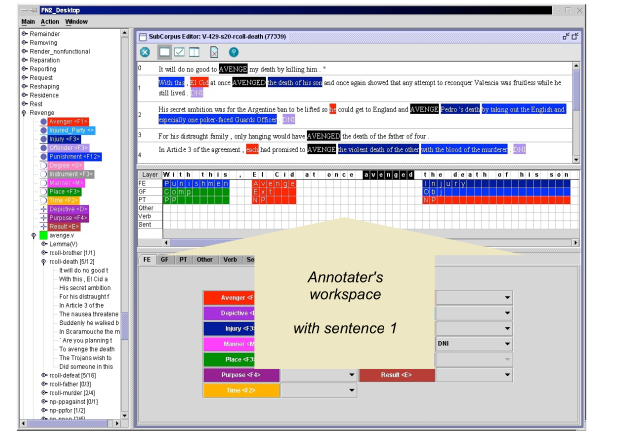
\includegraphics[scale=0.8]{03/framenet.png}
    \caption{Esempio di visualizzazione di FrameNet con il Frame Revenge.}
\end{figure}

\paragraph{Due tipologie di target:}

\begin{itemize}
  \item \fancyglitter{Predicati:} parole che evocano frames, creano contesti per le informazioni da inserire. L'obiettivo dell'annotazione è trovare gli argomenti.
  \item \fancyglitter{Fillers:} parole che soddisfano ruoli semantici nei frames evocati dai predicati. L'obiettivo dell'annotazione è identificare il frame e FE della frase.
\end{itemize}

\nt{Tipicamente parole diverse nello stesso frame mostrano variazione in come gli FE sono realizzati grammaticamente.}

\dfn{Valenza}{
La valenza è il numero e il tipo degli argomenti controllati da un predicato.
}

\paragraph{La valenza può essere di vario tipo:}

\begin{itemize}
  \item Impersonale. 
  \item Intransitiva. 
  \item Transitiva. 
  \item Ditransitiva. 
  \item Tritransitiva.
\end{itemize}

\qs{}{Nel frame Revenge attraverso quali significati sintattici è realizzato l'offender?}

\begin{itemize}
  \item Come un oggetto diretto. 
  \item Con la preposizione \textit{on}. 
  \item Con \textit{against}. 
  \item Con \textit{with}. 
  \item Con \textit{at}.
\end{itemize}

\qs{}{Quale FE è espressa dall'oggetto di avenge?}

\begin{itemize}
  \item L'injured\_party. 
  \item L'injury.
\end{itemize}

\paragraph{Altre definizioni:}

\begin{itemize}
  \item \fancyglitter{Copertura lessicale:} tutte le parole importanti associate con ogni frame. 
  \item \fancyglitter{Combinatorica:} tutti i patterns sintattici in cui ogni parola serve per esprimere il frame.  
  \item \fancyglitter{Dati di frequenza:} non sono collezionati direttamente da FrameNet.
\end{itemize}

\subsection{Frame Semantics e Text Understanding}

\paragraph{Information extraction:}

\begin{itemize}
  \item Si vuole progettare un'applicazione per estrarre informazioni dalle notizie di un giornale. 
  \item I dati di FrameNet dovrebbero poter essere usati per: 
    \begin{itemize}
      \item WSD. 
      \item Composizione semantica. 
      \item Scelta tra possibili alternative analisi sintattiche. 
      \item Attivazione di un vocabolario topic-related. 
    \end{itemize}
\end{itemize}

\paragraph{Risoluzione dell'anafora:}

\begin{itemize}
  \item \fancyglitter{Pronominale:} ci si riferisce a un referente con un pronome. 
  \item Frasi nominali definite: l'antecedente si riferisce a una frase con "$<$the$><$noun$ phrase>$". 
  \item Quantificatori/Ordinali: l'anafora è quantificata come "uno" e ordinalizzata come "primo".
\end{itemize}

\paragraph{Principi di utilizzo:}

\begin{itemize}
  \item Si può scegliere una parola per capire quali frame possano essere attivati da quella parola. 
  \item Identificati i ruoli semantici si cerca di accoppiare le necessità semantiche di ogni frame attivato con le porzioni della frase in input. 
  \item Il frame che si adatta meglio è quello scelto.
\end{itemize}

\paragraph{Disambiguazione:}

\begin{itemize}
  \item I significati possono essere inferiti mediante un criterio di coerenza. 
  \item FN non li fornisce direttamente, ma offre descrizioni di frame collegati e legami semantici tra le parole per facilitare i giudizi.
\end{itemize}

\paragraph{Blocchi di più parole:}

\begin{itemize}
  \item L'analisi non può procedere sulla base delle parole prese una alla volta. 
  \item È riconosciuto lo stretto legame tra le parole.
\end{itemize}

\paragraph{Altre cose:}

\begin{itemize}
  \item L'autore di un articolo può aggiungere informazione testimoniale a una parte della descrizione. 
  \item Esistono frame metalinguistici.
\end{itemize}
